% 来源：OEBPS/Text/Section0001_split_007.xhtml#sigil_toc_id_48

\BookChapter{35}
\section[第35章\q 沃伦·巴菲特：奥马哈圣人]{第35章\\ 沃伦·巴菲特：奥马哈圣人}

\begin{figure}[htbp]
\centering
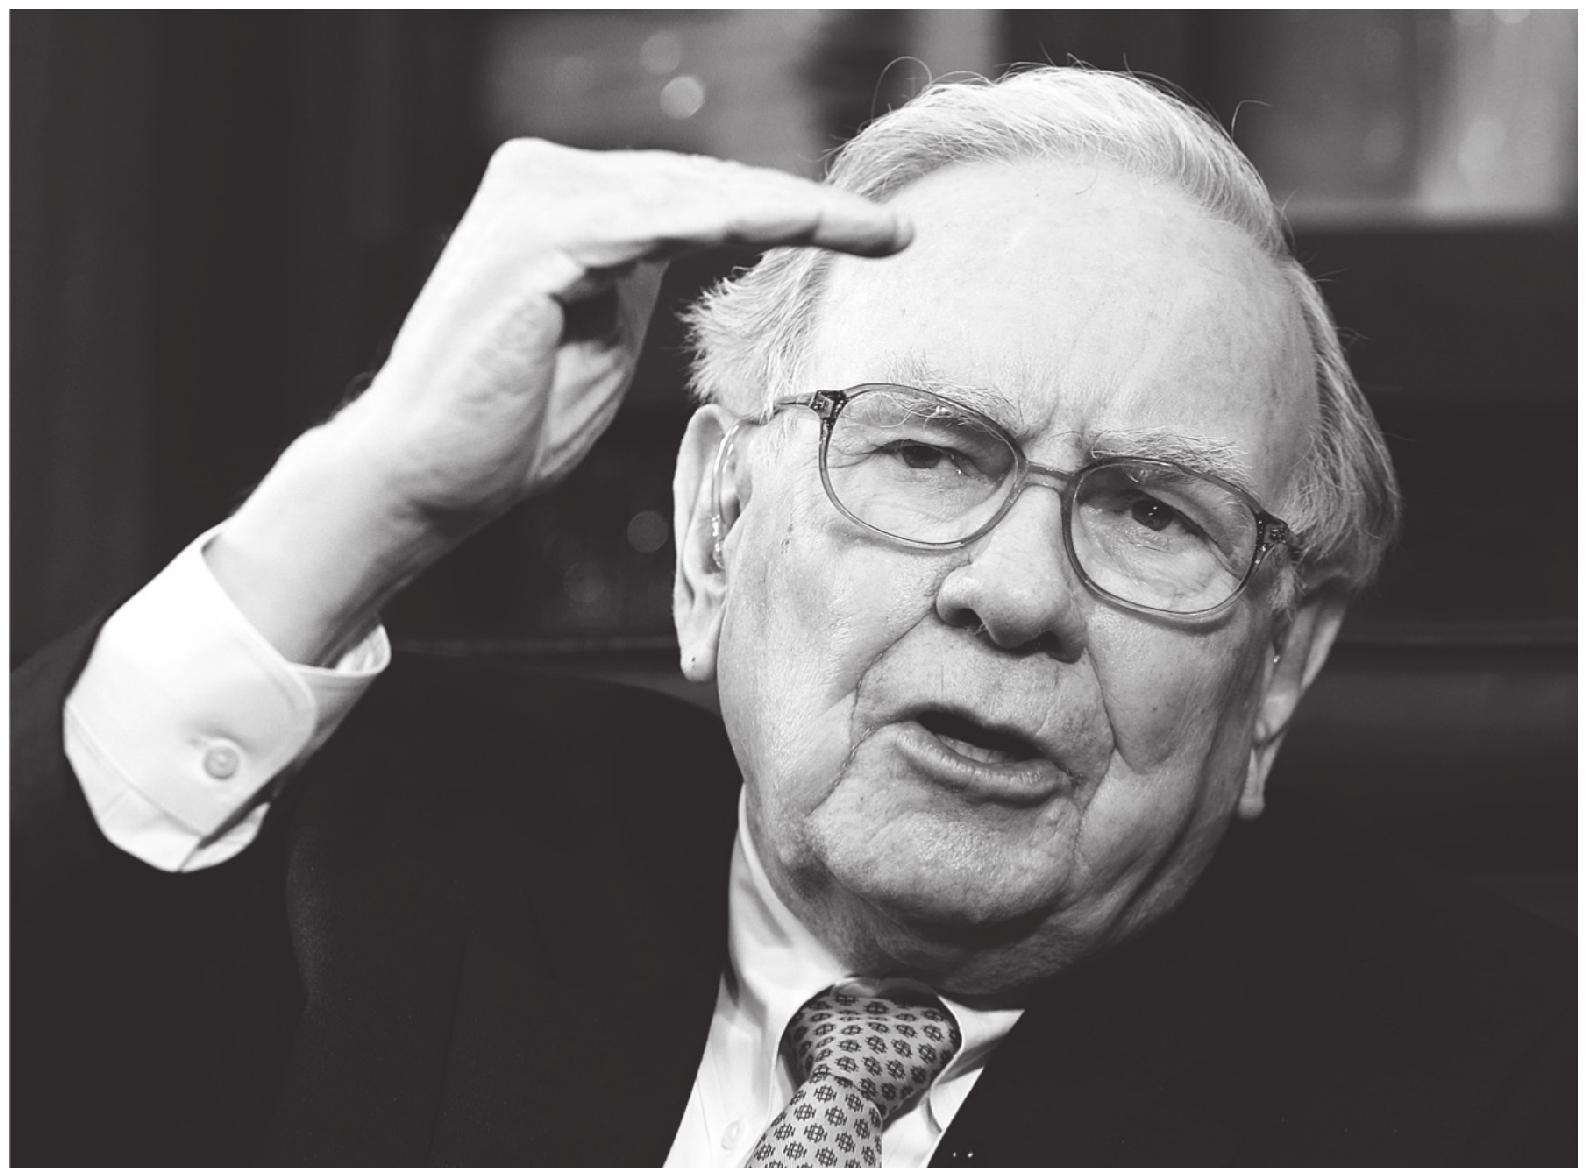
\includegraphics[width=0.55\linewidth,keepaspectratio]{image/沃伦·巴菲特肖像.jpg}
\caption*{沃伦·巴菲特}
\end{figure}

投资传奇大师，伯克希尔–哈撒韦公司首席执行官

我坐在美国《今日秀》节目的休息室里，等着开始录节目，这时一个人独自走了进来：沃伦·巴菲特，20世纪最伟大的投资人之一，个人财富676亿美元，世界排名第三的富豪。按照节目安排，我们一起参加圆桌讨论会，还包括Spanx内衣创始人萨拉·布雷克里，将要担任白宫住房和城市发展部部长的朱利安·卡斯特罗，以及主持人马特·劳尔。我们要一起讨论经济，谈谈我们对美国经济发展方向的看法。跟全球数以百万计的投资者一样，我一直是巴菲特的超级粉丝，他白手起家的故事深深地打动了我。巴菲特当初不过是内布拉斯加州一个不起眼的股票经纪人，后来做投资，收购了新英格兰地区一家失败的纺织企业伯克希尔–哈撒韦公司，并将其一步一步地发展成为全球市值第五大的上市公司。它资产规模近5000亿美元，投资控股很多家公司，业务种类繁多，从GEICO汽车保险公司到喜诗糖果公司，几乎你能想到的业务它全都有。巴菲特的投资成功之道并不那么神秘，就是价值投资：这套投资体系是他从导师格雷厄姆那里学来的，他不断完善，发扬光大，使其日臻完美。价值投资策略的核心是寻找价值被市场过于低估的公司，然后买进股票，预期这家公司的股价长期来看会上涨，回归到其价值水平。这是一种最简单的风险—收益不对称的投资机会，它要求你要花费很多时间和精力进行研究分析，要求你有相当高的研究分析和投资技能，还要求你手上有相当多的现金，这也正是为什么巴菲特一直追寻收购保险公司的机会，因为保险公司能够产生巨大的现金流，手上有了规模巨大的资金，巴菲特才能抓住巨大的投资机会。

巴菲特不但在商业投资上取得了非凡的成功，还成为有史以来慷慨捐赠最多的慈善家，他发誓要把个人财富的99\%都捐赠给慈善事业，他把这些资金委托给比尔·盖茨夫妇的慈善基金会，以用于慈善事业。在企业领导人里面，巴菲特说的话可能是得到引用次数最多的。你在本书里也会时不时地读到巴菲特的名言，这些都是他的智慧结晶，对于投资者来说都是无价之宝。

我发现，我的投资偶像巴菲特竟然和我同处一室，这么好的向大师求教的机会，我怎能错过？我赶紧上前打招呼，自我介绍，告诉他我正在写书的事。我问道：“巴菲特先生，我们能不能找个时间坐一下，请您谈谈，在现在这个波动性很大的经济情况下，个人投资者应当怎么做才能在投资比赛中获胜？”

巴菲特看着我，眼睛眨了几下，明显在思考。然后他微微一笑，说：“托尼，我很想帮你，但是关于这个主题，能说的东西我都已经说过了。”

巴菲特说的这个理由，我很难跟他争论。从1970年开始，巴菲特每年都要在年报里写一封致股东的信，大家都热切期待。巴菲特致股东的信，语言朴实无华，他给出投资建议，评论经济形势和企业经营，字字珠玑。除此之外，封面上印有巴菲特名字的书有50多种，甚至其中几本还是巴菲特本人写的。

不过，我还是想再试一试。

“但是，既然你现在已经公开宣布，要把绝大部分财富都捐赠给慈善事业，那么你会给你的家人推荐什么样的投资组合，让他们自己的投资得到安全保值，并且不断增值？”

巴菲特一听，又微微一笑，抓住我的胳膊。“很简单。”他说，“投资指数基金，这是一条阳光大道，让你能够投资伟大的美国企业，不用像购买公募基金那样付给基金经理很高的管理费，一直持有这些伟大企业的股票，长期下来，你就会赢。”

哇！全世界最有名的选股高手，已经欣然接受了指数基金，巴菲特公开说，对于绝大多数个人投资者来说，指数基金是最好的投资工具，也是最有成本效率的投资工具。

后来，我还找了史蒂夫·福布斯和瑞·达利欧两位好友，帮我劝沃伦·巴菲特接受一次更加细致深入的交谈，他传话给我，没有必要。巴菲特告诉我，关于投资最重要的事，他想说的，在致股东的信里都说过了，印成白纸黑字随着年报公开披露。他想告诉个人投资者的东西，浓缩起来就是一句话：投资指数基金，让你能够分散范围很广的整个股票市场，同时持有那些全球最优秀公司的股票，购买指数基金之后，你只要一直持有它很多年就行了。我明白了！在2014年致股东的信中，巴菲特再次特别强调了他给所有投资者的建议：投资指数基金。巴菲特的资产配置是什么样的？下面是巴菲特留给他妻子的投资指令，巴菲特要求他去世之后他的信托资产做如此投资：

“10\%放在美国短期国债上，90\%放在成本非常低的标准普尔500指数基金上。（我建议投资先锋公司的标准普尔500指数基金。）我相信，按照这个投资方针执行的话，这个信托资产的长期业绩会胜过大多数投资者——那些购买基金支付很高费用给基金经理的投资者。不管是养老基金这样的机构投资者还是个人投资者，长期业绩都会大幅落后于指数基金。

约翰·博格听到这些肯定会非常高兴！美国最受尊敬的投资大师对约翰·博格近40年来一直推广的指数基金，表示完全认同和支持，而且会直接使用。

别忘了，巴菲特下了100万美元的大赌注，赌指数基金长期能够战胜对冲基金。和巴菲特对赌的对手是位于纽约的门徒伙伴公司，专门为客户精选对冲基金。巴菲特发起的赌局是：门徒伙伴公司精选出5只顶级对冲基金的平均业绩，不能战胜巴菲特选择的先锋标准普尔500指数基金，赌期是10年，从2008年1月1日到2017年12月31日。2014年1月，赌局已经过去了6年，标准普尔500指数上涨了43.8\%，而门徒伙伴公司挑选的那5只对冲基金平均业绩为12.5\%，巴菲特大幅领先。

你听到了吗？奥马哈的投资圣人已经说过了：最好的投资方法是买入并长期持有指数基金！
